
% LaTeX-pohja Jyväskylän Kemian Laitoksen kandi- ja maisteritutkielmiin. Seuraa kemian laitoksen "Tieteellisen opinnäytetyön kirjoitusohje" -dokumentit muotoiluohjeita mahdollisimman tarkasti

% Versio 1.0, 2026/02/11

% License:  lppl  lppl1   lppl1.3 lppl1.3c

% Kirjoittajat:
% Alkuperäinen versio: Toni Kiljunen
% Uusin kattava päivitys ja Overleaf-pohja: Marko Melander, Minttu Smith & Toni Kiljunen


%\documentclass[a4paper, 12pt, finnish, twoside]{article}
\documentclass[a4paper, 12pt, finnish]{article}
\usepackage[T1]{fontenc}
\usepackage[finnish]{babel}
\usepackage{graphicx}
\usepackage{epstopdf}
\usepackage{booktabs}
\usepackage{amsmath, amssymb} % matematiikkaa varten
\usepackage{stmaryrd}
\usepackage{icomma}
\usepackage{physics} % kätevä paketti yhtälöille
\usepackage{url} % www-osoitteille
\usepackage[symbol]{footmisc} % alaviitteille
% asettelu
\usepackage[top=2.5cm, bottom=1.5cm, inner=2.5cm,outer=2.5cm]{geometry}
 \setlength{\headheight}{14.5pt}
\usepackage{tikz}
\linespread{1.3}
\parindent0pt
\parskip1.5ex
\usepackage{fancyhdr}
\fancyhf{}
\fancyhead[C]{\thepage}
\pagestyle{fancy}
\renewcommand{\headrulewidth}{0pt}
\usepackage[margin=10pt, labelfont=rm, labelsep=period]{caption}

% linkkien muotoilu
\usepackage{hyperref}
\hypersetup{
    colorlinks,
    linkcolor={black},
    citecolor=black,
    urlcolor={black}
}
\usepackage[utf8]{inputenc}
\usepackage{graphicx} 		% Add graphics capabilities
\usepackage{amsmath}  		% Better maths support	
\usepackage{chemfig} % rakenteille
\usepackage{graphicx}     % 
\usepackage{tikzducks} % Paketti place-holder -ankkakuviin
\usepackage{booktabs}     % muotoiluja ja fontteja varten
\usepackage{amsmath}
\usepackage{amssymb}
\usepackage{stmaryrd}
\usepackage{icomma}     % suom. desimaalipilkkua varten matikkamoodissa
\usepackage[dvipsnames]{xcolor}
\usepackage[version=3]{mhchem}     % kemiallisia kaavoja vaten
\usepackage{lipsum} % pseudoteksti
\usepackage{minted} % koodin esittämiseen
\usemintedstyle{vs} % minted-muotoilu

% viitteiden muotoilu kemian laitoksen "Tieteellisen opinnäytetyön kirjoitusohje" mukaisesti
\usepackage{csquotes}
\usepackage[style=jyu-chem-thesis, doi=true, backend=biber]{biblatex} % aseta doi=false palautettavaan versioon

%%%%%%%%%%%
% Viitteiden muotoilu loppuu
%%%%%%%%%%%

\addbibresource{jyu-chem-thesis.bib} % tiedosto, jossa viitteet ovat
\renewcommand\refname{Viitteet}


\renewcommand{\contentsname}{Sisällysluettelo}

\newcommand*{\otsikko}{\fontsize{18pt}{22pt} \bf \fontfamily{phv}\selectfont} %Ympäristö tutkielman otsikon fontille, Helvetica 18 pt

\usepackage[version=3]{mhchem}

\makeatletter
\newcounter{reaction}
\renewcommand\thereaction{R\arabic{reaction}}
\newcommand\reactiontag{\refstepcounter{reaction}\tag{\thereaction}}
\newcommand\reaction@[2][]{\begin{equation}\ce{#2}%
\ifx\@empty#1\@empty\else\label{#1}\fi%
\reactiontag\end{equation}}
\newcommand\reaction@nonumber[1]{\begin{equation*}\ce{#1}%
\end{equation*}}
\newcommand\reaction{\@ifstar{\reaction@nonumber}{\reaction@}}
\renewcommand\@biblabel[1]{#1.}
\makeatother
\newcommand{\onlinecite}[1]{\hspace{-1 ex} \nocite{#1}\citenum{#1}}
\renewcommand{\thepage}{\roman{page}}

%%%%%%%%%%%%%%%%%
% tästä alkaa itse dokumentti
%%%%%%%%%%%%%%%%%%

\begin{document}

% kansilehti
\begin{titlepage}
\tikz[remember picture,overlay] \node[opacity=0.99,inner sep=0pt] at (current page.center){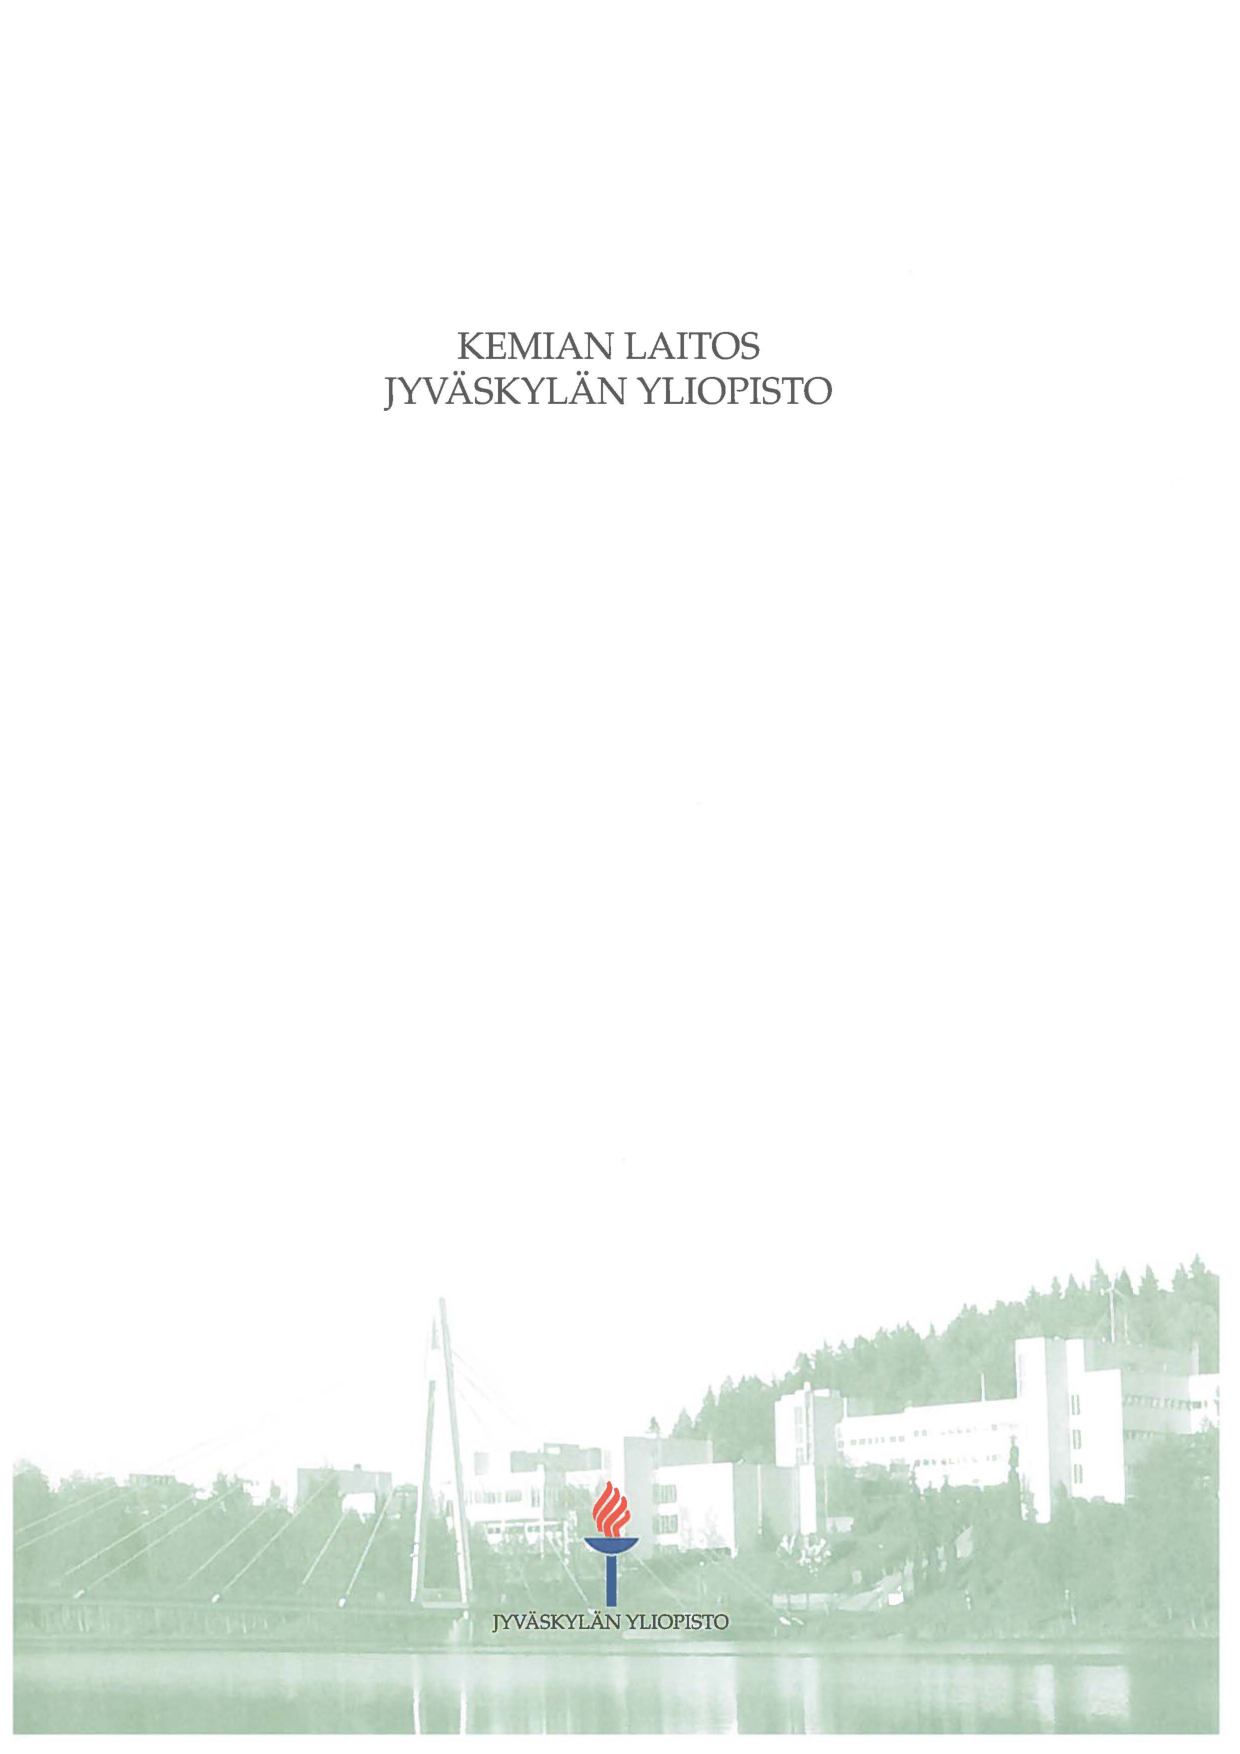
\includegraphics[width=\paperwidth,height=\paperheight]{jyu-chem-thesis-background.pdf}};
\vspace{10cm}
\begin{center}
\otsikko{Tutkielman otsikko}
%{\Huge {\bf Tutkielman otsikko}}
\end{center}
\vskip 4cm
\begin{flushleft}
%\hspace{7cm} Jyv\"askyl\"an yliopisto \\ % ei tarvita, kun
%\hspace{7cm} Kemian laitos \\ % käytössä kansilehtipohja
\hspace{9cm} {\fontfamily{phv}\selectfont Kandidaatintutkielma ja -projekti\\
\hspace{9cm} 02.02.2020\\
\hspace{9cm} Malli Oppilas}
\end{flushleft}
\end{titlepage}
%\thispagestyle{empty}
\newpage \setcounter{page}{2}
\mbox{}
\newpage

\section*{Tiivistelmä}
\addcontentsline{toc}{section}{Tiivistelmä}
tekstiä

\newpage
\section*{Esipuhe}
\addcontentsline{toc}{section}{Esipuhe}
tekstiä

\newpage
\section*{Käytetyt lyhenteet ja vieraskieliset termit}
\addcontentsline{toc}{section}{Lyhenteet ja vieraskieliset termit}
\begin{table}[h!]
\begin{tabular}{lll}
\textbf{Lyhenne} & \textbf{Merkitys} & \textbf{Suomennos}\\
\hline
AES     & atomic emission spectroscopy & atomiemissiospektroskopia\\
ANOVA   & analysis of variance & varianssianalyysi\\
CE      & circular economy & kiertotalous\\
CRM     & critical raw material & kriittinen raaka-aine\\
EDX     & energy-dispersive & energiadispersiivinen\\
ICP     & inductively coupled plasma & induktiivisesti kytketty plasma\\
LoD     & limit of detection & havaintoraja\\
LoQ     & limit of quantification & määritysraja\\
OES     & optical emission spectroscopy & optinen emissiospektroskopia \\
REE     & rare-earth element & harvinainen maametalli\\
SCM     & shrinking core model & kutistuvan ytimen malli\\
SEM     & scanning electron microscopy & pyyhkäisyelektronimikroskopia\\
XRF     & x-ray fluorescence & röntgenfluoresenssi\\
\end{tabular}
\end{table}
\newpage
\thispagestyle{empty}
\tableofcontents
\cleardoublepage
\pagenumbering{arabic}



\newpage

\section{Johdanto}

Alla lyhyet ohjeet sekä näppäriä vinkkejä LaTeXin käyttöön opinnäytetöissä.


\subsection{Yhtälöitä ja taulukko}

Alla esimerkkejä yhtälöiden ja taulukoiden käytöstä.

Reaktion kertaluku määritetään integroitujen nopeuslakien avulla, esimerkiksi
% ei tyhjaa riviä, jottei tule kappalejakoa
\begin{equation} \label{eq:eq0}
[\mathrm{A}_2\mathrm{B}_3](t) = -k_\mathrm{r} t + [\mathrm{A}_2\mathrm{B}_3]_0 \,,
\end{equation}
% 
jossa $k_\mathrm{r}$ on reaktion nopeusvakio ja $[\mathrm{A}_2\mathrm{B}_3]$ ajasta $t$ riippuva konsentraatio. 
Yhtälöstä~(\ref{eq:eq0}) % "sitova välilyönti"
nähdään, että nollannen kertaluvun reaktiossa konsentraation tulisi noudattaa suoran yhtälöä \cite{atkins}. 

Ensimmäinen ja toinen kertaluku voidaan linearisoida seuraavien yhtälöiden mukaisesti:
\begin{align} 
 \ln [\mathrm{A}_2\mathrm{B}_3] &= -k_\mathrm{r} t + \ln [\mathrm{A}_2\mathrm{B}_3]_0  \label{eq:eq1} & \text{(1. kl)}\,, \\
 \frac{1}{[\mathrm{A}_2\mathrm{B}_3]} &= k_\mathrm{r} t + \frac{1}{[\mathrm{A}_2\mathrm{B}_3]_0}  \label{eq:eq2} & \text{(2. kl)} \,.
\end{align}
Esittämällä konsentraatio yhtälöiden~(\ref{eq:eq0})--(\ref{eq:eq2}) mukaisesti voidaan päätellä mitä kertalukua reaktio noudattaa ja määrittää vastaava reaktion nopeusvakion arvo. Taulukossa~\ref{tab:esimtable} on yhtälöiden~(\ref{eq:eq0})--(\ref{eq:eq2}) perusteella lasketut arvot graafista esitystä varten. 
Taulukoiden tekemistä voi helpottaa huomattavasti käyttämällä sivustoa \url{https://www.tablesgenerator.com}, jonka avulla taulukon muotoilut saa tehtyvä helposti ja tiedot saa tuotua esimerkiksi Excelistä.

\begin{table}[!hbtp] \begin{center}
\caption{\label{tab:esimtable} Konsentraation aikariippuvuus. Reaktion kertaluvun määrittämiseen tarvittavat arvot}
\begin{tabular}{rccc}
\hline\hline  % tai \toprule
$t$ (s) & [A$_2$B$_3$] (mol dm$^{-3}$) & $\ln [\mathrm{A}_2\mathrm{B}_3]$ & $ [\mathrm{A}_2\mathrm{B}_3]^{-1}$ (dm$^3$ mol$^{-1}$)\\
\hline % tai \midrule
0 & 0,100 & $-2{,}303$ & 10,0 \\
50 & 0,067 & $-2{,}703$ & 14,9 \\
jne &  &  & \\
\hline\hline % tai \bottomathrmule
\end{tabular}\end{center}
\end{table}

\newpage
\subsection{Kemialliset yhdisteet ja rakenteet}

LaTeXissa on paljon hyödyllisiä paketteja kemiallisten yhdisteiden ja rakenteiden tekemiseen. Esimerkiksi yhdisteet voi kirjoittaa näin \ce{C2H5OH} tai ioneille \ce{Na+Cl-}. Reaktiot taas hoituvat näin käyttämällä reaction-funktiota, jonka formaatti seuraa mhchem-pakettia.

\reaction{Nu- + E+ \to NuE} % ka


Joitain rakenteita voi myös piirtää chemfig-paketilla, ks. kuva~\ref{fig:kofeiini}.

\begin{figure}[!ht]
    \centering
    \chemfig{*6((=O)-N(-)-(*5(-N=-N(-)-))=-(=O)-N(-)-)}
    \caption{Kofeiinin rakenne. Muista, että kuvatekstien tulee olla informatiivisia ja kuviin tulee olla viittaus tekstissä.}
    \label{fig:kofeiini}
\end{figure}


\subsection{Physics-paketti}

Yhtälöissä voi myös käyttää näppärää physics-pakettia, joka helpottaa yhtälöiden kirjoittamista. Esimerkiksi kvanttimekaaninen odotusarvo voidaan kirjoittaa seuraavasti käyttäen Diracin notaatioita:
%
\begin{equation}
    \expval{A} = \mel{\Psi}{\hat{A}}{\Psi} \,.
\end{equation}
%
Vastaavasti esimerkiksi osittaisderivaatat hoituvat kätevästi. Tässä esimerkki sisäenergian kokonaisdifferentiaalille:
%
\begin{equation}
    \dd U(T,V)= \left(\frac{\partial U}{\partial T}\right)_{V}\dd T
    +\left(\frac{\partial U}{\partial V}\right)_{T}\dd V
    =C_V\dd T+\pi_T \dd V \,.
\end{equation}

\subsection{Kuvia}

Wrapfig-komennolla kuvan voi halutessaan laittaa myös tekstin joukkoon. Esimerkki on esitetty kuvan~\ref{fig:kuva} avulla.

\begin{figure}[!ht]
    \centering\includegraphics[width=0.5\linewidth]{example-image-b}
    \caption{Esimerkki wrapfig-toiminnon käytöstä.}
    \label{fig:kuva}
\end{figure}


\subsection{Lähdekoodi}

Halutessaan työn joukkoon voi laittaa myös lähdekoodia, jota on käytetty projektissa. Usein nämä tiedot annetaan liitetiedostoissa. Esimerkiksi:
\begin{minted}{python}
import numpy as np
print('Small Python test')
\end{minted}


\section{Viittaamisesta}

Testataan tässä viittaamista artikkeliin,~\cite{PhysRev.136.B864, 10.1063/5.0182685} ohjeisiin,~\cite{ohje} WWW-sivuun~\cite{iupac} ja opinnäytetyöhön~\cite{thesis} käyttämällä yläindeksiä.\footnote{WWW-sivuihin viitataan @online-tietueella ja opinnäytetyöhön @thesis-tietueella. Ks. viitteet.bib esimerkkinä muotoilusta.} Lisäksi voidaan viitata tarvittaessa "riviviitteellä" näin \citeinline{ohje}. Tällaista tarvitaan esimerkiksi kuvateksteissä tai taulukoiden alaviitteinä, jos vaikka halutaan ilmaista, että tiedot ovat viitteestä \citeinline{ohje}. 

%Samalla kannattaa varmistaa, että viitteiden muotoilu on oikein.

Huomioi, että lehtien nimet eivät (ainakaan toistaiseksi) tule automaattisesti CASSI-mukaiseen lyhennettyyn muotoon. Tämän voi korjata manuaalisesti muokkaamalla viitteet.bib -tiedoston "journal"-tietueessa olevan lehden nimen sen lyhenteellä.


\section{Yhteenveto}

Loppu.

\newpage
\addcontentsline{toc}{section}{Viitteet}
\printbibliography[title=Viitteet]

\newpage
\section*{Liitteet}
\addcontentsline{toc}{section}{Liitteet}

\begin{itemize}
\itemindent=5mm
    \item[Liite 1:] Liitteen seliteteksti 
    \item[Liite 2:] jne.
\end{itemize}

%Huomaa että sivunumerointi ei jatku liitteisiin. Tuo liitteet include-toiminnolla ja katkaise sivunumerointi \thispagestyle{empty}

\end{document}